\scanpage{81}
% The typed block is upside down relative to the notes. Two long pen strokes traverse the sheet.
\handwritten{$V\subset C$ \quad $\deleted{\unsure{\Lambda\ \mathrm{et}\ \Lambda}}$}

\[
\handwritten{\begin{aligned}
&\unsure{i|j}_{*}(\Lambda)_V=\Lambda_C &&1+\unsure{e'|C'|\varepsilon'}\\
&\mathbb R^1i_*(\Lambda_V)=\text{\uuline{$\unsure{{\mu_\infty^{-1}}_{Z,C}|\mu_{\infty_{Z,C}}^{-1}}$}} &&\unsure{\mathrm{EP}|\mathrm{TP}|\pm P}(C)
\end{aligned}}
\]
\handwritten{2.14.}

\handwritten{\diagram{\begin{tikzcd}[ampersand replacement=\&]
\unsure{\overline Y|\widetilde Y}\arrow[r]\arrow[d,no head] \& \unsure{\overline X|\widetilde X}\arrow[d,no head]\\
Y\arrow[r,no head] \& X
\end{tikzcd}\qquad
\begin{tikzcd}[ampersand replacement=\&]
{} \& X'\arrow[d,"p"] \& p_*(F)\\
F \& X \& {}
\end{tikzcd}}}

\handwritten{\diagram{\begin{tikzcd}[ampersand replacement=\&]
\overline Y\arrow[r,no head,"\overline h"']\arrow[d,no head,"p_Y"'] \& \overline X\arrow[d,no head,"p"] \& \overline F\\
Y\arrow[r,"h"'] \& X \& {}
\end{tikzcd}}}
\[
\handwritten{h^*({\unsure{\mathbb R|\mathrm R}}^1p_*(\unsure{\overline F|F}))\longrightarrow\mathbb R^1p_{Y*}(\overline h^*(\overline F))}
\]

\figure{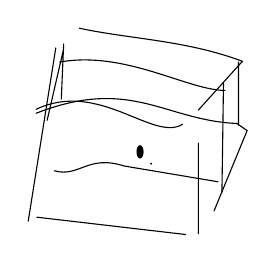
\begin{tikzpicture}[x=1cm,y=1cm,line cap=round]
\draw (0,0) -- (.35,2.2) (.24,1.28) -- (.45,2.19) (.42,1.55) -- (.45,2.25);
\draw (.65,2.45) .. controls (1.30,2.31) and (2.0,2.30) .. (2.72,2.03) -- (2.16,1.41);
\draw (.40,2.02) .. controls (1.23,2.17) and (2.03,1.66) .. (2.50,1.66);
\draw (2.67,2.02) -- (2.67,1.22) (2.48,1.76) -- (2.46,.36);
\draw (.10,1.42) .. controls (.9,1.8) and (1.59,1) .. (1.96,1.23);
\draw (.10,1.37) .. controls (1.31,1.84) and (1.73,1.28) .. (2.65,1.24) -- (2.78,1.15) -- (2.36,.13);
\draw (.33,.64) .. controls (.65,.55) and (.75,.85) .. (1.22,.70) -- (2.41,.50);
\draw (.11,.05) -- (2.00,-.17) (2.16,-.16) -- (2.16,.99);
\fill (1.42,.88) ellipse (.045 and .085);\fill (1.56,.73) circle (.014);
\end{tikzpicture}}

\figure{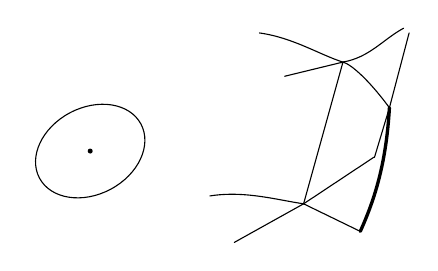
\begin{tikzpicture}[x=1cm,y=1cm,line cap=round]
\draw[rotate around={28:(0,0)}] (0,0) ellipse (.73 and .55);\fill (0,0) circle (.032);
\draw (2.15,1.5) .. controls (2.58,1.44) and (2.92,1.22) .. (3.21,1.13) .. controls (3.55,1.19) and (3.72,1.42) .. (3.98,1.56);
\draw (2.47,.95) -- (3.21,1.13) -- (2.71,-.67) -- (1.83,-1.16);
\draw (1.52,-.57) .. controls (1.96,-.5) and (2.37,-.62) .. (2.71,-.67) -- (3.43,-1.02);
\draw (2.71,-.67) -- (3.60,-.08) (3.21,1.13) .. controls (3.32,1.10) and (3.55,.89) .. (3.80,.55);
\draw (4.05,1.5) -- (3.80,.55) -- (3.61,-.08);
\draw[very thick] (3.80,.55) .. controls (3.76,-.14) and (3.62,-.60) .. (3.43,-1.02);
\end{tikzpicture}}

% Typed passage, read after turning the sheet through 180 degrees.
\deleted{\uline{Corollaire} 6.3. Supposons que $T^{\bullet},T'^{\bullet}$ proviennent de foncteurs cohomologiques (dénotés par les mêmes symboles) sur la catégorie dérivée droite $D^+(C)$, à valeurs dans $C'$ (les notations étant par ailleurs celles de 6.2., mais on ne suppose pas nécessa\deleted{\unsure{r}}irement $T^i$ effaçable pour $i\quad 0$). On suppose la condition 6.2. a) satisfaite.}

\deleted{(i) Soit $K^{\bullet}$ un complexe dans $C$, à degrés bornés inférieurement, et tel que $H^i(K^{\bullet})=0$ pour $i\quad 0$. Alors $\phi^i(K^{\bullet}):T^i(K^{\bullet})\qquad T'^{i}(K^{\bullet})$ est un isomorphisme pour $i\quad n$, un monomorphisme pour $i=n+1$.}

\deleted{(ii) Soit $u:L^{\bullet}\qquad K^{\bullet}$ un homomorphisme de complexes à degrés bornés inférieurement, tel que $H^i(u):H^i(L)\qquad H^i(K^{\bullet})$ soit un isomorphisme pour $i\quad 0$, un monomorphisme pour $i=0$. \deleted{\unsure{Alors} $\unsure{\phi^i}$ \illegible{1}}}
% archive sheet number: 80
